\chapter{clean} \label{clean}

\section{Introduction}

An LPE may contain redundant information, for example because some of its summands contain all behavior of other summands or because some of its summands will never be (or become) enabled.
Obviously, such summands can be removed without hesitation, which may result in a speedup in other computations in which the LPE is input.

The \texttt{clean} command attempts to detect redundant summands and removes the ones that it finds.
The state space of the LPE is not affected by the changes.

\section{Formal background}

\subsection{Summand containment}

Consider two summands, $s_\alpha$ and $s_\beta$, and reference their elements conform \ref{summandelements}.

Summand $s_\alpha$ is said to \emph{contain} $s_\beta$ if these two conditions hold:

\begin{itemize}
\item $s_\alpha$ and $s_\beta$ must communicate over the exact same channel with exactly as many channel variables; that is, $C_\alpha = C_\beta \land m_\alpha = m_\beta$.

\item Define the mapping
\begin{align*}
X_\alpha = [x_\beta(j) \rightarrow x_\alpha(j) \;|\; 1 \leq j \leq \text{min}(m_1, m_2)]
\end{align*}

The following conditions must also hold:
\begin{align*}
g_\beta[X_\alpha] &\rightarrow g_\alpha \\
v_\alpha(p) = v_\beta(p)[X_\alpha] &\leftrightarrow \text{\textit{True}} \text{ for all } p \in [p_1, \cdots{}, p_k]
\end{align*}

The first condition demands that whenever $s_\beta$ is enabled, $s_\alpha$ must also be enabled; consequently, $s_\alpha$ is `always ready' to perform the same behavior as $s_\beta$.
The second condition demands that the state after the application of $s_\alpha$ is the same as the state after the application of $s_\beta$, regardless of the values of communication variables and LPE parameters.
\end{itemize}

Note that $s_\alpha$ could contain all behavior of $s_\beta$ without these two conditions being true (we under-approximate by tolerating false negatives)!

\subsection{Summand reachability}

Consider summands $s_\alpha$ and $s_\beta$, referencing their elements conform \ref{summandelements}.
Summand $s_\alpha$ is said to be a \emph{possible predecessor} of $s_\beta$ if the following expression \emph{could be} satisfiable:
\begin{align*}
g_\alpha \land {g_\beta}[v \rightarrow q(v) \;|\; v \in \varsof{g_\beta} \setminus P][p \rightarrow v_\alpha(p) \;|\; p \in P]
\end{align*}

where $q(v)$ is a bijective function that relates variable $v$ to a fresh variable.

A summand $s_\beta$ is said to be \emph{reachable} if at least one of these conditions holds:

\begin{itemize}
\item It is possible that summand $s_\beta$ is enabled in the initial state of the LPE.
Formally, $s_\beta$ is reachable if the LPE is initialized as
\begin{align*}
P(v_I(p_1), \cdots{}, v_I(p_m))
\end{align*}

and if
\begin{align*}
g_\beta[p \rightarrow v_I(p) \;|\; p \in P]
\end{align*}

\emph{could be} satisfiable.

\item There exists at least one other summand $s_\alpha$ in the same LPE that is a possible predecessor of $s_\beta$.
It is \emph{not} sufficient if the only possible predecessor of $s_\beta$ is $s_\beta$ itself!
\end{itemize}

Summand reachability is \emph{over-approximated}.
For example, if it is uncertain whether a summand is enabled in the initial state, the summand is considered to be reachable.

\section{Algorithm}

The algorithm consists of 2 phases.

In the first phase, the algorithm does a pairwise comparison of all summands of the LPE.
If it discovers that some summand $s_1$ contains another summand $s_2$, it removes $s_2$ from the LPE.

In the second phase, the algorithm starts by determining which summands are reachable in the initial state of the LPE (the first condition for reachability in the previous section).
This becomes the initial value of the set $X$.
Then, until a fixpoint is reached, to $X$ all summands are added of which there exists a possible predecessor in $X$.
The output LPE of the algorithm contains all summands that are in the fixpoint of $X$.

\section{Example}

Consider the following LPE:

\begin{lstlisting}
//Process definition:
PROCDEF example[A :: Int](x :: Int)
  = A ? i [[x==0]] >-> example[A](1)
  + A ? j [[x==1]] >-> example[A](2)
  + A ? k [[x==1]] >-> example[A](2)
  + A ? l [[x==2]] >-> example[A](0)
  + A ? m [[x>=2]] >-> example[A](0)
  ;

//Initialization:
example[A](0);
\end{lstlisting}

The \texttt{clean} command will detect that the second and third summands of the LPE are equivalent and remove one of them.
It will also detect that the fifth summand contains the fourth summand, and therefore remove the fourth summand.

Now consider

\begin{lstlisting}
//Process definition:
PROCDEF example[A :: Int, B](x :: Int)
  = A ? i [[i != 13]] >-> example[A, B](i)
  + B [[x == 13]] >-> example[A, B](x)
  ;

//Initialization:
example[A, B](0);
\end{lstlisting}

The second summand is unreachable: it is not enabled in the initial state (since \texttt{x = 0}) and it is never enabled after the application of the first summand (since \texttt{i != 13}).

\section{Benchmark results}

The following durations were measured with a benchmark for several models:
\begin{itemize}
\item The average duration of \txs{} to make 500 steps in a model without converting it to LPE form or applying LPE operations;
\item The average duration of \txs{} to make 500 steps in a model after it has been converted to LPE form;
\item The average duration of \txs{} to make 500 steps in a model after it has been converted to LPE form and after the \texttt{clean} operation has been applied.
\end{itemize}

When plotting the second series of measurements against the first (see Figure~\ref{lpe-only-vs-original:fig}), the following conclusions can be drawn:
\begin{itemize}
\item The effect of the LPE transformation on performance is negative in most cases.
\item The effect of the LPE transformation on performance is positive in some cases, but not dramatically so.
\item For one model (\texttt{Adder3}), the effect of the LPE transformation is extremely positive (5.2 seconds instead of 12.5).
Unfortunately, this model is not very realistic since it simply consists of three parallel processes without any synchronization.
\end{itemize}

\begin{figure}[!ht]
\begin{center}
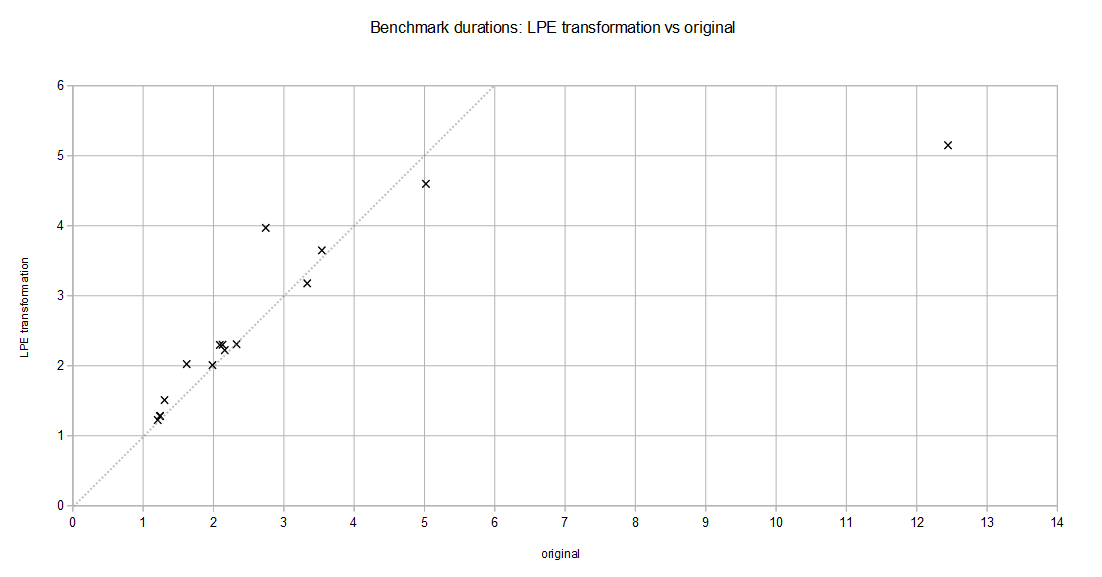
\includegraphics[width=0.8\linewidth]{charts/lpe-only-vs-original}
\caption{Benchmark results: LPE transformation vs original}
\label{lpe-only-vs-original:fig}
\end{center}
\end{figure}

It is possible that the \texttt{clean} operation has a significant positive influence on the performance of \txs{}.
Based on a plot of the third series of measurements against the second (see Figure~\ref{clean-vs-lpe-only:fig}), however, this cannot be concluded: only part of the models show slight (but significant) improvements, whereas other models suffer an (also slight) additional performance loss.

\begin{figure}[!ht]
\begin{center}
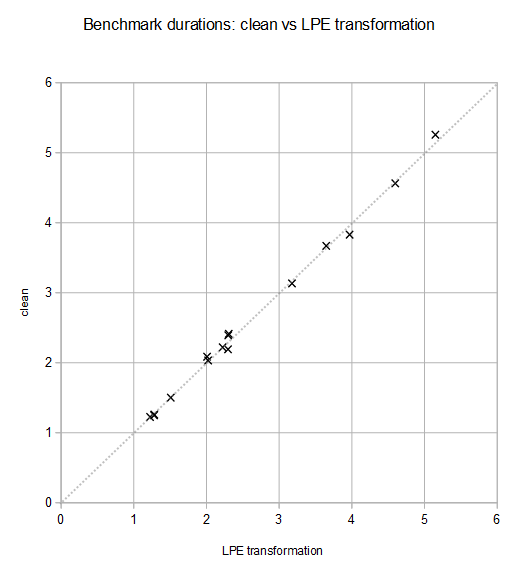
\includegraphics[width=0.5\linewidth]{charts/clean-vs-lpe-only}
\caption{Benchmark results: clean vs LPE transformation}
\label{clean-vs-lpe-only:fig}
\end{center}
\end{figure}



